\chapter{AX.25}

AX.25 is the amateur radio derivative of CCITT X.25 that was designed during the early 1980's 
as the primary data link protocol used by amateur packet networks.
The AX.25 specification has been maintained by the Tucson Amateur Packet Radio (TAPR) 
organization until its latest release, Version 2.2 in July of 1998. 

The most significant difference between AX.25 and the original X.25 protocol lies
in the hardware addesses used by AX.25 based on each station's FCC issues callsign. 
Each node is addresses by their FCC callsign plus an additional 4 bit 
secondard station identifier (SSID), which allows each licensee to maintain and operate 
up to 16 stations in each packet namespace.

\section{FCC Identification Requirements}

One of the advantages of using a station's FCC callsign as part of the addressing protocol
is that it additionally fulfills the FCC requirement to identify every transmitting station
every ten minutes per Title 47 CFR \S97.119. \S97.119 is unfortunately vague and archaic as
to the exact requirements for this identification every ten times during a transmision. No
definitive judgements were found by the author as to 
the actual legal implications of the following protocol
for identifying operating stations, and this section must not be interpreted as any form of
legal advice on a station's legal identification requirements.

Source stations are identified during every transmission by including an ASCII representation
of their FCC callsign in the source address field of their AX.25 frames. 
Each Digipeater that subsequentlu handles this third party traffic may identify by appending 
their callsign to the packet's routing path and ensuring that it is the last valid FCC callsign
marked as ``consumed" as will be explained in section~\ref{subsec:ax25RoutingPath}.

The two exceptions to this rule are what are called non-trace digipeaters which do not
append their callsign to a packet's routing path and any station which uses a tactical callsign
instead of their FCC-issued callsign. Tactical callsigns are often used for packet stations to
give them more meaningful addresses than their control operator's callsign. One example of where
tactical callsigns are often used is events where APRS is used to track support vehicles that 
already have tactical callsigns issued to their voice operators, such as ``SAG-3" or ``CHASE-1."
Since these stations do not use their FCC callsign as part of their AX.25 address,
these stations do need to somehow ensure that they transmit their callsign 
at least once every ten minutes while operating, which
may be accomplished by including the control operator's callsign in the comment text of an 
originating APRS beacon.

\section{Header Format for APRS}

A very limited subset of the complete AX.25 protocol is used by APRS due to APRS 
deliberately avoiding the use of any of the connected or control modes of AX.25. This 
means that any AX.25 protocol stack used for APRS need only support unconnected information (UI)
frames per the AX.25 specification.

\begin{figure}
	\centering
	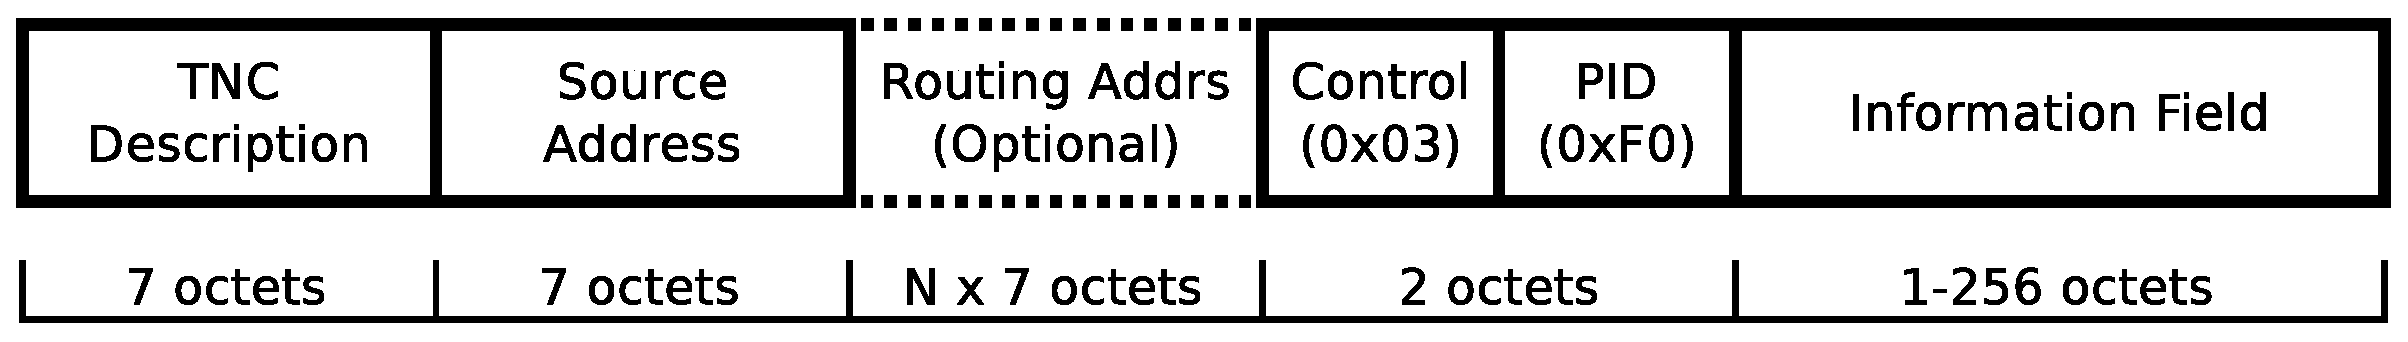
\includegraphics[width=1.0\textwidth]{src/dia/ax25ui}
	\caption{AX.25 UI Packet Format}
	\label{ax25uiformat}
\end{figure}

\subsection{TNC Description / Destination Address}

Traditional AX.25 traffic is usually directed at a single station, which would be indicated by 
a packet's destination address. Since APRS is strictly a one-to-many network protocol at layer 3, this field
is not needed for APRS and has been overloaded for several different applications.

The most popular application for this field is to be used as a tracker identifier, where a
six character identifier is allocated from the APRS Working Group to identify a specific 
APRS TNC and firmware version. Experimental trackers which have not yet received a tracker ID
should use the APZ??? identifier.

\subsection{Source Address}

The source address is the FCC or tactical callsign used by the beaconing APRS station, with an 
additional SSID appended to the station, which may range from zero to 15. Source addresses must 
be at least three characters long, and may not be any longer than six. Stations using AX.25 
over RF are limited to the SSID's of -0 to -15 due to AX.25's binary format, 
while stations using alternative data link transports may use any 
two alphanumeric characters for their SSID.

\subsection{Routing Path}
\label{subsec:ax25RoutingPath}

The AX.25 routing path is an optional variable-length field consisting of an ordered list of
digipeaters which should process and retransmit the considered packet. Should a station not
require the use of this field, it can be completely omitted and the end-of-path bit should be
set on the source address field. The path must consist of an integer number of seven octets.

The original AX.25 version 2.0 spec allowed for anywhere from zero to eight digipeaters to
be included in an AX.25 frame. Unfortunately, due to the unreliable nature of amateur 
packet radio, packets with a routing path requesting as many as eight hops would rarely be 
successfully delivered to the end station, so the version 2.2 specification for AX.25 was
rewritten limiting the number of requested digipeaters to two with the argument that packets
traveling beyond two hops should be handled by a higher layer protocol than AX.25.
This limitation, and the unclear figure 3.1 which indicates that only zero or two digipeaters
are allowed, are both ignored by APRS, which allows the original eight digipeater path, but
users are strongly discouraged from using beyond three hops on the national network.

\subsection{Control Flags}

The Control Flag octet indicates what type of AX.25 frame the considered packet is. 
Since APRS stictly uses only Unconnected Information (UI) frames, this field must
contain the value of 0x03.

\subsection{Protocol IDentifier}

The Protocol IDentifier (PID) field is normally used to identify the layer three protocol
being transported by AX.25. TAPR has reportedly stopped processing requests for new PID
values to be issued to new layer 3 applications of AX.25 \cite{millernopid}, 
so APRS uses the value of
0xF0 indicating that no layer 3 protocol is in use.

\subsection{Information Field}

The rest of the AX.25 frame contains the APRS payload in what is called the Information field.
The end of the Information field is indicated by the layer 1 modulation, which is traditionally
the Bell 202 FCS and 0x7E flag.

